\documentclass[11pt]{article}
\usepackage[margin=1in]{geometry}
\usepackage{graphicx}
\usepackage{array}
\usepackage{booktabs}
\usepackage{tabularx}
\usepackage{caption}
\usepackage{hyperref}
\usepackage[square,authoryear]{natbib}

\newcolumntype{Y}{>{\raggedright\arraybackslash}X}
\captionsetup{font=small,justification=justified,singlelinecheck=false}

\title{Institutional Robustness in Sequential Commons}
\author{Ameer Alhashemi}
\date{\today}

\begin{document}
\maketitle

\begin{abstract}
Renewable commons provide a controlled setting for comparing governance arrangements under strategic pressure. Earlier results in Fishery Commons show that central interventions can be ranked under repeated adversarial strategy injection, with adaptive quotas emerging as the strongest signal in the medium tier. Earlier results in Harvest Commons show that local-only, central-only, and hybrid governance differ under stronger search-based pressure, and that hybrid governance ranks first in the confirmatory architecture matrix. The present study re-evaluates Harvest under three literature-backed scenario archetypes and two oversight regimes that introduce imperfect detection, delayed enforcement, limited targeting capacity, and governance budget cost. The ranking of architectures varies across scenarios. Hybrid governance ranks first throughout the community-irrigation scenario and under ideal forest co-management, whereas top-down-only governance ranks first in constrained forest co-management and in the higher-pressure regulated-fishery setting. These results support a comparative reading of governance architecture in which rankings depend on scenario structure and implementation constraints.
\end{abstract}

\section{Introduction}

\subsection{Existing Work}

Sequential commons provide a controlled setting for studying governance when individual incentives can damage a shared resource. The classical common-pool resource literature identifies the same problem in fisheries, irrigation systems, forests, and other renewable resources: open access and weak institutions are associated with overuse even when long-run collective welfare would favour restraint \citep{gordon1954common, scott1955fishery, ostrom1990}. Later work links institutional performance to monitoring, incentives, local participation, and the relation between local and higher-level authority \citep{hilborn2005, gutierrez2011, ostrom1993, ostrom1994, villamayor2020, nagendra2012}. These studies provide the substantive basis for comparing local, central, and mixed governance arrangements in shared-resource settings.

Sequential social-dilemma and multi-agent benchmark work develops this problem in computational environments. These benchmarks make it possible to study repeated interaction, partner composition, learning dynamics, and held-out social settings in a controlled way \citep{leibo2017multiagent, meltingpot2021, socialjax2025}. They are useful for identifying failures that do not appear in single-agent evaluation. A policy can perform well in isolation and still be associated with poor collective outcomes once other agents respond strategically or once the environment rewards short-term extraction.

Scalable oversight studies a related problem from a different direction. Work on scalable oversight asks how a weaker overseer can evaluate, guide, or check a stronger system, and how oversight performance changes as the capability gap widens \citep{bowman2022oversight, engels2025scaling}. The methodological lesson for this study is that oversight should not be treated as perfect by default. Detection, intervention capacity, delay, and cost can be included as evaluation conditions.

Recent work on LLM-generated populations adds a further motivation for studying changing strategic populations. Willis, Du, and Leibo study language-model-generated strategies in a social dilemma, and Willis, Zhao, Du, and Leibo scale this idea to larger populations with cultural evolution \citep{willis2025cooperation, willis2026collective}. Their results report systematic differences in cooperative behaviour across model-generated strategies and poor collective outcomes under some population dynamics. The present paper uses this concern about changing populations to motivate adversarial turnover in a commons benchmark; direct evaluation of LLM strategy populations is left for later work.

\subsection{Research Question}

The research question is: which governance architectures remain robust in sequential commons when stronger adversarial strategies repeatedly enter the population and oversight is imperfect? The study focuses on governance architecture instead of a single learned policy. The comparison covers bottom-up-only, top-down-only, and hybrid governance, with a no-governance condition used as a baseline in the broader evidence chain.

The study evaluates this question in Harvest Commons. Harvest is re-evaluated under three literature-backed scenario archetypes corresponding to regulated fishery, community irrigation, and forest co-management. Oversight is represented through four implementation constraints: imperfect detection, delayed enforcement, limited targeting capacity, and governance budget cost. In operational terms, these constraints act through the government agent. They determine whether an intended cap is detected, when it becomes active, how many agents can be targeted in one step, and what cost is charged when intervention occurs.

The empirical result is a scenario-dependent comparison of governance architecture under explicit oversight frictions. Community-irrigation settings favour hybrid governance under both ideal and constrained oversight. Constrained forest co-management and the higher-pressure regulated-fishery setting favour top-down-only governance. The benchmark reports how architecture rankings vary when adversarial turnover is retained and oversight quality is varied directly.

\section{Methods}

\subsection{Prior Studies}

The analysis builds on two earlier studies.

First, Fishery Commons provides the simpler signal-design study from the earlier stage of the project. It is a minimal renewable commons with one shared stock, per-agent harvest actions, regeneration, and collapse dynamics. Earlier experiments compared no governance, monitoring with sanctions, adaptive quotas, and temporary closures under repeated adversarial strategy injection. The matched baseline used two injector families: mutation and live model-generated JSON strategies produced through Ollama with qwen2.5:3b-instruct. In that simpler setting, the benchmark already showed that central interventions can be ranked under escalating strategic pressure.

Second, Harvest Commons serves as the architecture benchmark developed in the later stage of the project. Harvest extends the commons problem from one global stock to local renewable patches with local interaction, optional communication, and optional side-payments. Across the broader project, the architecture space includes a no-governance baseline together with bottom-up-only, top-down-only, and hybrid governance. Earlier results restored the full architecture spectrum, ran a high-power confirmatory comparison under a strong search-based adversary, added welfare-incidence logging, and organized non-LLM attackers into a capability ladder. The attacker ladder used four injector families in increasing order of strength: random, mutation, adversarial heuristic, and search over mutations. Those results remain part of the evidence base for this paper.

\subsection{Scenario Archetypes}

Three scenario presets are used. The regulated-fishery preset represents centralized monitoring, quotas, and enforcement under ecological uncertainty \citep{hilborn2005, gutierrez2011}. The community-irrigation preset represents local rule enforcement and user monitoring in self-governing irrigation systems \citep{ostrom1993, ostrom1994, villamayor2020}. The forest-co-management preset represents mixed local stewardship and higher-level intervention in polycentric forest governance \citep{nagendra2012}. The parameter values define benchmark archetypes drawn from those institutional settings. They are chosen to distinguish recognizable governance forms within Harvest rather than to reproduce any individual case numerically.

\begin{table}[t]
  \centering
  \caption{Scenario preset values used in the institutional-friction extension.}
  \label{tab:scenario_presets}
  \footnotesize
  \renewcommand{\arraystretch}{1.08}
  \begin{tabular*}{\linewidth}{@{\extracolsep{\fill}}>{\raggedright\arraybackslash}p{3.0cm}c>{\raggedright\arraybackslash}p{2.1cm}cccc@{}}
    \toprule
    Scenario & Tier & Mix & Regen. & Spill. & Comm & Credit \\
    \midrule
    Regulated fishery & Med. & Balanced & 0.70 & 0.10 & Off & Off \\
    Community irrigation & Med. & Balanced & 0.64 & 0.15 & On & Off \\
    Forest co-management & Hard & Adv. heavy & 0.56 & 0.22 & On & On \\
    \bottomrule
  \end{tabular*}
\end{table}

\subsection{Governance Architecture and Oversight Frictions}

Harvest remains the main environment for the extension. The governance conditions are none, bottom-up only, top-down only, and hybrid. The institutional-friction module keeps those conditions fixed and adds four oversight frictions: detection recall, enforcement delay, maximum targeted share, and governance budget cost. Two regimes are compared. The ideal regime reproduces frictionless governance. The constrained regime introduces incomplete detection, one-round delays, capped targeting capacity, and a per-intervention budget cost.

\begin{table}[t]
  \centering
  \caption{Oversight-regime values used in the institutional-friction extension.}
  \label{tab:oversight_regimes}
  \small
  \renewcommand{\arraystretch}{1.08}
  \begin{tabularx}{\linewidth}{@{}>{\raggedright\arraybackslash}p{2.1cm}YYYY@{}}
    \toprule
    Regime & Detection recall & Delay rounds & Max target share & Budget cost \\
    \midrule
    Ideal & 1.0 & 0 & 1.0 & 0.00 \\
    Constrained & 0.7 & 1 & 0.5 & 0.02 \\
    \bottomrule
  \end{tabularx}
\end{table}

\subsection{Extension Scope}

The extension evaluates three governance architectures with central intervention: bottom-up-only, top-down-only, and hybrid governance. These architectures are compared across the three scenario presets and two oversight regimes. The full design spans thirty-six evaluated cells and one hundred and eighty run-level replicates.

Architectures are ranked within each experimental cell by lexicographic order on three aggregate outcomes: lower garden failure, then higher patch health, then higher welfare. A garden-failure event occurs when more than half of the local patches remain below four resource units for five consecutive steps. This is the same ranking rule used in the earlier Harvest architecture study.

\section{Results}

\subsection{Prior Results}

Earlier Fishery and Harvest results in the same project provide the empirical baseline. Fishery Commons provides the narrower signal-design result. In the matched baseline, monitoring with sanctions reduces held-out collapse relative to no governance under both mutation-based injection and live model-generated JSON strategy injection. In the broader non-LLM top-down sweep, adaptive quotas emerge as the strongest overall central signal in the medium tier, while temporary closures remain a credible ecological fallback.

Harvest Commons provides the stronger baseline architecture claim. In the restored four-condition pilot, bottom-up-only governance is empirically distinct from the no-governance baseline but remains ecologically weaker than architectures with central intervention. In the high-power confirmatory matrix, hybrid governance ranks first in all eight decision cells under the failure-then-patch-health-then-welfare rule. Relative to top-down-only governance, hybrid improves patch health in all eight cells, is non-worse on neighborhood overharvest in six of eight, and incurs a moderate mean welfare delta of \(-0.1363\). Relative to bottom-up-only governance, both architectures with central intervention buy large ecological gains at substantially larger welfare cost.

\begin{figure}[t]
  \centering
  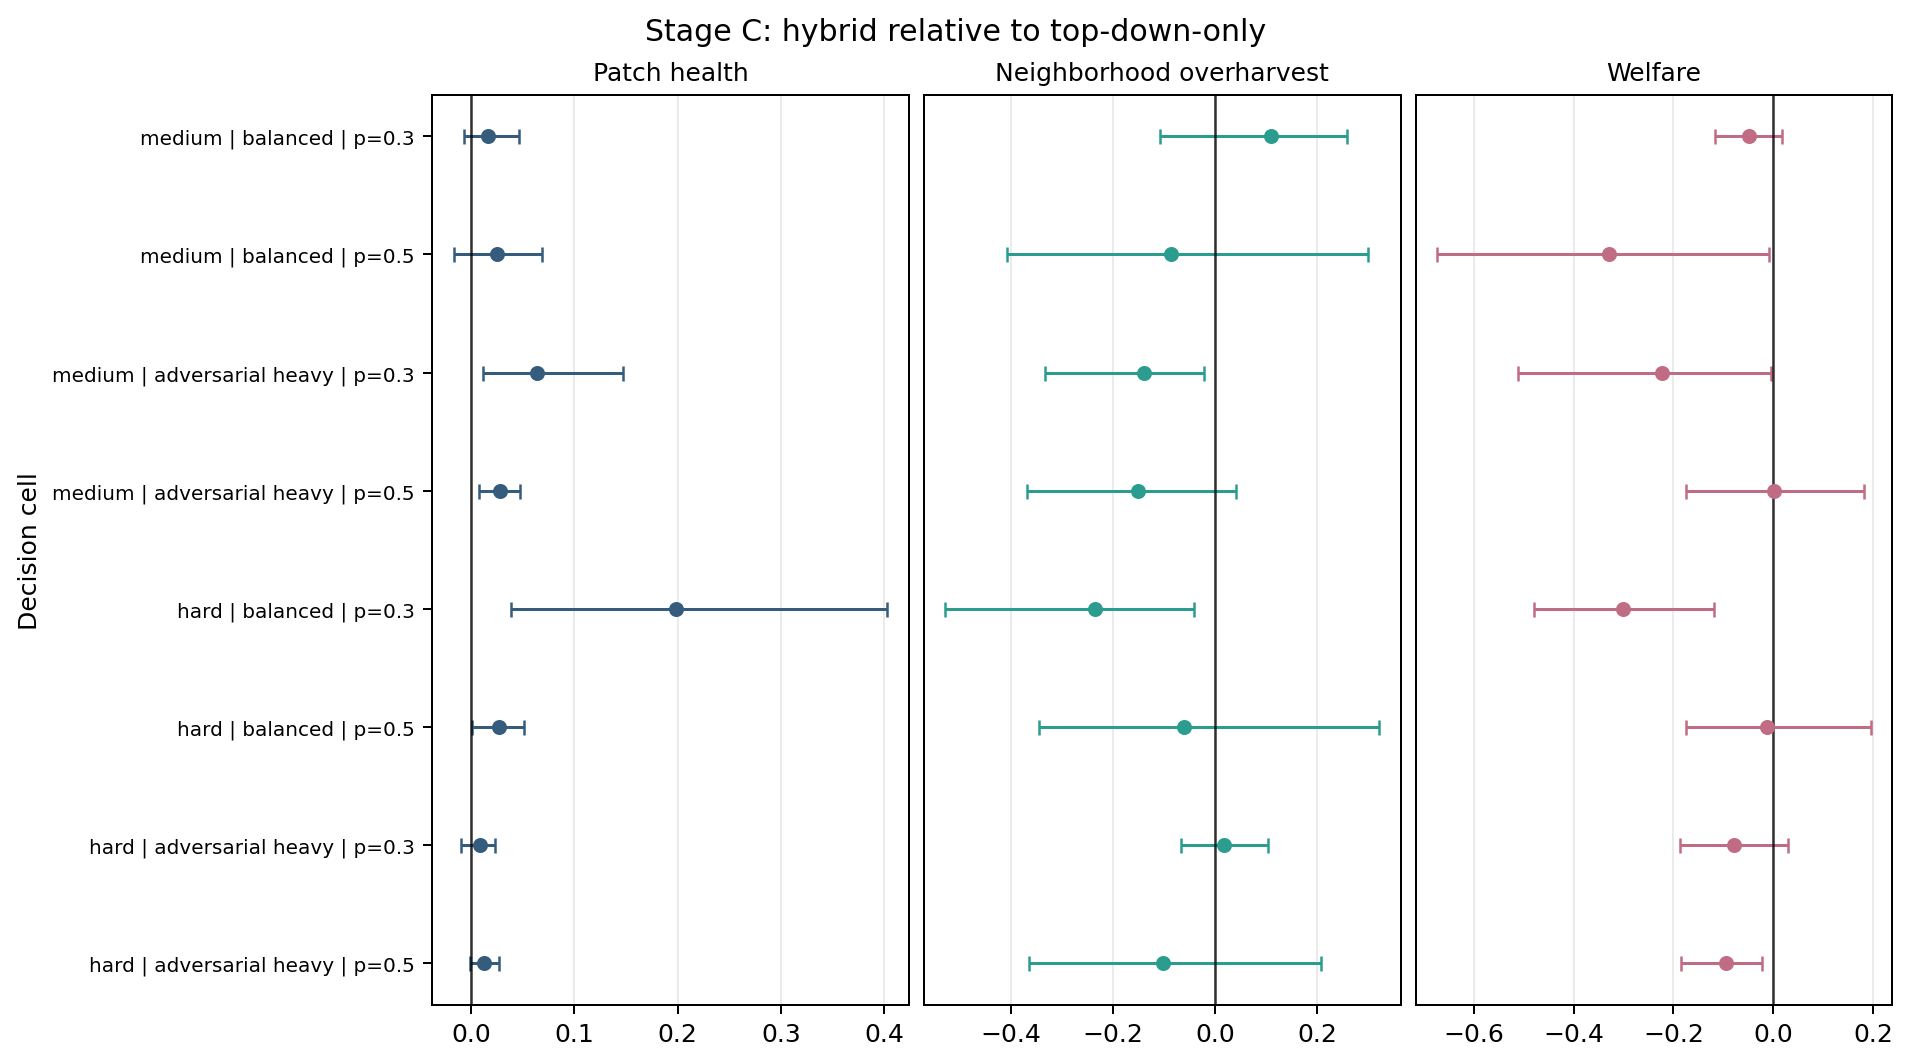
\includegraphics[width=\linewidth,trim={0 0 0 1.25cm},clip]{figures/harvest_architecture_stageC_architecture.png}
  \caption{Baseline Harvest architecture effect sizes from the confirmatory architecture matrix. Under the failure-then-patch-health-then-welfare rule, hybrid governance ranks first in all eight confirmatory cells while improving patch health in every cell relative to top-down-only control.}
  \label{fig:baseline_stagec_architecture}
\end{figure}

The capability ladder and welfare-incidence analyses sharpen that baseline result. Across the 32 ladder cells, hybrid governance ranks first in 25 and top-down-only governance ranks first in 7, while both governed architectures retain a stable ecological advantage over bottom-up-only governance throughout the non-LLM attacker ladder. The incidence summaries show that the additional welfare cost of moving from top-down-only to hybrid governance is modest relative to the much larger penalty associated with restoring ecological control over local-only governance. Figures~\ref{fig:baseline_stagec_architecture} and~\ref{fig:baseline_capability_ladder} are regenerated from the frozen result bundles used in the earlier studies.

Taken together, the carried-forward evidence establishes three points that matter for the extension. Fishery Commons shows that central interventions can be ranked under repeated strategic turnover. The confirmatory Harvest matrix provides a strong baseline result for hybrid governance before oversight frictions are introduced. The capability ladder and welfare-incidence analyses show that architectures with central intervention remain ecologically stronger than local-only governance even when the ordering between hybrid and top-down-only governance becomes more contested.

\begin{figure}[t]
  \centering
  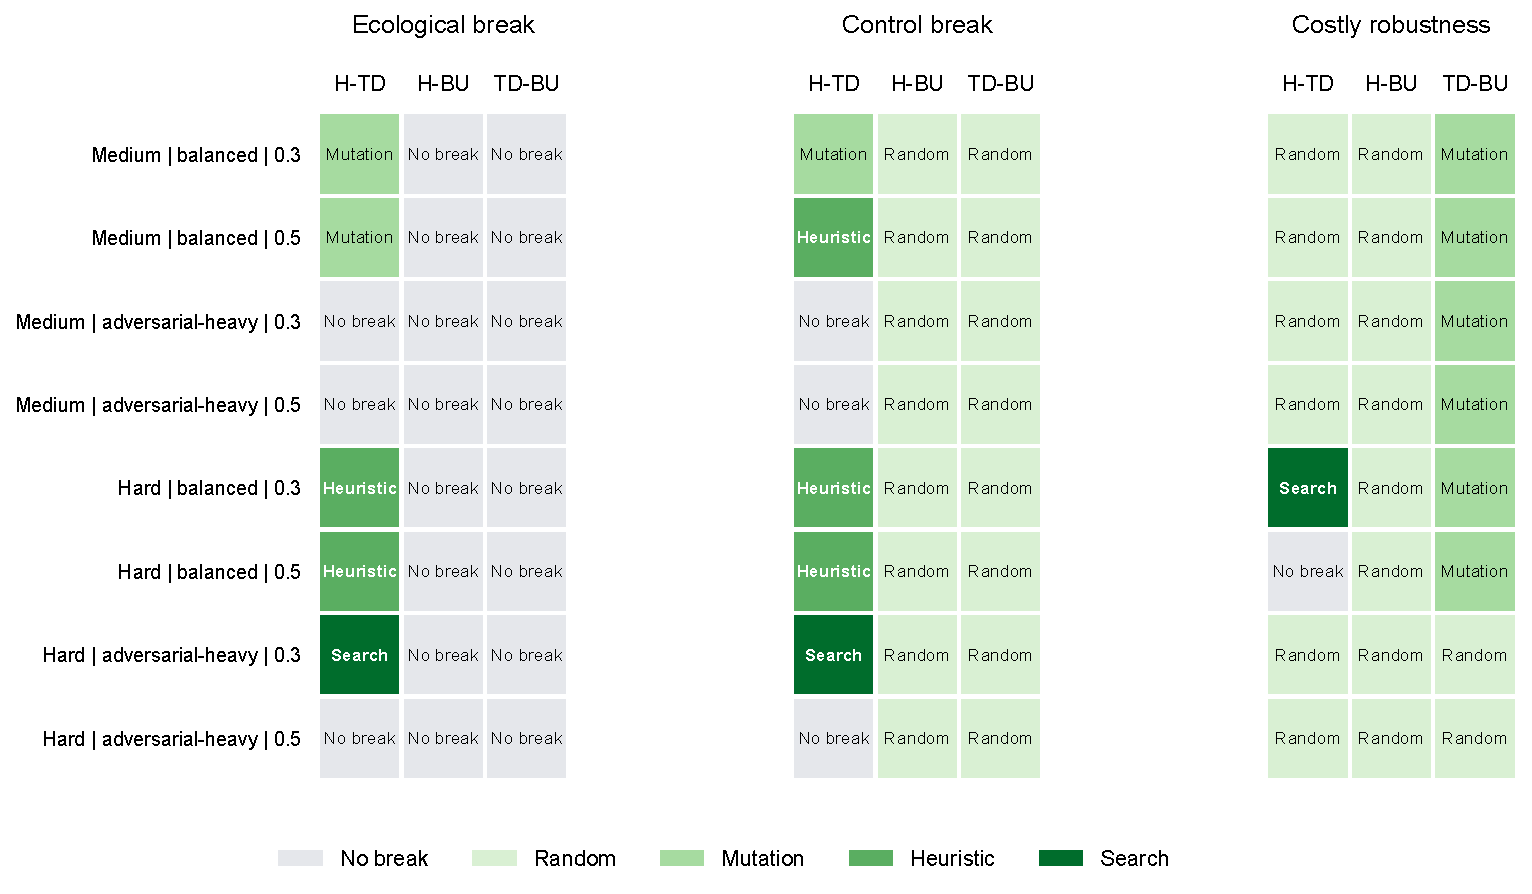
\includegraphics[width=\linewidth]{figures/harvest_capability_ladder_stageB_publication.pdf}
  \caption{Baseline Harvest capability ladder from the existing evidence base. The main split remains between architectures with central intervention and local-only governance, while the ordering between hybrid and top-down-only governance becomes more contested as attacker strength rises.}
  \label{fig:baseline_capability_ladder}
\end{figure}

\subsection{Architecture under institutional frictions}

Harvest is then re-evaluated under the three scenario archetypes and two oversight regimes. The main comparison remains hybrid versus top-down-only governance, with bottom-up-only governance retained as the decentralized comparison case.

The results vary across scenarios. In the community-irrigation scenario, hybrid governance ranks first in all four tested cells, under both ideal and constrained oversight, and records positive patch-health deltas against top-down-only governance in every case. In forest co-management, hybrid governance ranks first under ideal oversight, but top-down-only governance ranks first once oversight is constrained. In regulated fishery, the ranking depends on pressure: hybrid governance ranks first at the lower pressure level, whereas top-down-only governance ranks first at the higher pressure level in both oversight regimes.

Across all six scenario-pressure cells, the paired hybrid-minus-top-down-only contrast remains positive on patch health in five cells under ideal oversight and in five cells under constrained oversight. These ecological gains do not always translate into first-place ranking once welfare and control costs are included. Under ideal oversight, hybrid governance ranks first in five of the six cells. Under constrained oversight, it ranks first in three. The architecture ranking is therefore sensitive to scenario and oversight regime.

The decentralized baseline remains clearly weaker ecologically. Top-down-only governance exceeds bottom-up-only governance on patch health in every evaluated cell, and hybrid governance does the same. The cost of that ecological improvement is lower welfare relative to bottom-up-only governance, which remains the highest-welfare but least robust architecture. Figure~\ref{fig:moduleA_winner_map} summarizes the extension in a single winner map. Each cell shows the best-ranked architecture, while the annotated number reports the hybrid-minus-top-down patch-health difference.

\begin{figure}[t]
  \centering
  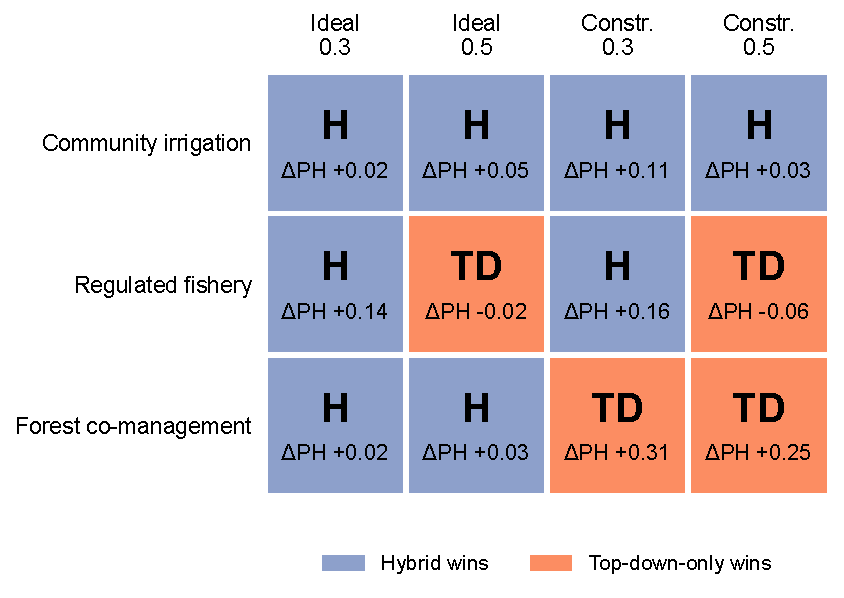
\includegraphics[width=0.88\linewidth]{figures/institutional_friction_winner_map.pdf}
  \caption{Compact summary of the institutional-friction extension. Cell color denotes the best-ranked architecture in each scenario, oversight regime, and pressure cell. The annotation reports the hybrid-minus-top-down patch-health difference, which shows where hybrid retains an ecological advantage even when it is not the overall winner.}
  \label{fig:moduleA_winner_map}
\end{figure}

\subsection{Scenario-Dependent Ranking}

The earlier confirmatory Harvest result showed that hybrid governance could outperform central-only control under stronger search-based pressure. The institutional-friction extension retains that result in some settings and reverses it in others. Once scenario structure and implementation frictions are introduced, the ordering between hybrid and top-down-only governance differs across cases. The resulting architecture ranking is scenario dependent.

\section{Discussion}

The institutional-friction results show that the ranking between hybrid and top-down-only governance depends on the scenario and on the practical limits of oversight. Community-irrigation settings favour hybrid governance most consistently. Constrained forest co-management and the higher-pressure regulated-fishery setting favour top-down-only governance.

These results narrow the scope of the earlier Harvest finding. The confirmatory architecture matrix still shows a strong result for hybrid governance under search-based pressure. After scenario structure and oversight frictions are introduced, that ordering no longer holds uniformly. The extension therefore changes the interpretation of the architecture comparison from a single ranking to a family of scenario-specific rankings.

The scenarios remain archetypal and are not calibrated to particular cases. The results support comparison across governance settings, but they should not be read as predictions for any one fishery, irrigation system, or forest governance arrangement. Each scenario family is represented by a single benchmark parameterization, and the institutional-friction extension fixes the attacker family to the strongest non-LLM search-based pressure instead of re-running the full attacker ladder within every new scenario.

Within those limits, the cumulative evidence is substantial. Fishery Commons ranks central interventions under repeated strategic turnover. Harvest Commons distinguishes local-only, central-only, and hybrid governance in a richer common-pool setting. The confirmatory architecture matrix, the capability ladder, the welfare-incidence analysis, and the institutional-friction extension together support a comparative claim about governance architecture under strategic pressure.


\clearpage
\bibliographystyle{plainnat}
\bibliography{refs}

\end{document}
